% !TeX program = latexmk
% !TeX root = dp-puzzle.tex
% Standalone DAC 2027 English manuscript.
% Edit this file and the local tables/, figures/, and references/ directly.
\documentclass[conference,10pt,letterpaper]{IEEEtran}
\usepackage[T1]{fontenc}
% IEEEtran supplies the standard conference fonts and page geometry.
% Existing vector figures use PDF 1.7. preserve their embedded fonts.
\pdfminorversion=7
\usepackage{amsmath,amssymb}
\usepackage{graphicx}
\usepackage[caption=false,font=footnotesize]{subfig}
\usepackage{booktabs}
\usepackage{cite}
\usepackage[hidelinks]{hyperref}
\graphicspath{{figures/}}
\newcommand{\PaperTitle}{DP-Puzzle: Exploring Throughput Ratios in Multi-Precision Tensor Cores with Composable Dot-Product Units}
\title{\PaperTitle}
\author{\IEEEauthorblockN{Anonymous Submission}}
\hypersetup{pdfauthor={},pdftitle={\PaperTitle},pdfsubject={English manuscript}}
\newcounter{DACreferencepage}
\AtEndDocument{%
  \ifnum\value{page}>\value{DACreferencepage}\relax
    \PackageWarningNoLine{DAC2027}{References exceed one page}%
  \fi}
\begin{document}
\bstctlcite{DPBSTcontrol}
\maketitle

% Queue Table I at the top of the first page's right column.
\suppressfloats[t]
% Opening-page industrial-ratio overview; automatic caption numbering.
\begin{table}[t]
\centering
\caption{Per-device dense matrix peaks (PFLOP/s) and roadmap targets}
\label{tab:vendor_ratios}
\begingroup\footnotesize\setlength{\tabcolsep}{2pt}
\begin{tabular*}{\columnwidth}{@{\extracolsep{\fill}}llrrrl@{}}
\toprule
Vendor & Product & BF16 & MXFP8 & MXFP4 & Ratio \\
\midrule
NVIDIA & B200 SXM~\cite{nvidiahgx}
 & 2.250 & 4.500 & 9.000 & \tpratio{1}{2}{4} \\
 & B300 SXM~\cite{nvidiahgx}
 & 2.250 & 4.500 & 13.500 & \tpratio{1}{2}{6} \\
 & Rubin GPU~\cite{nvidiaverarubin}
 & 4.000 & 17.500 & 35.000 & $\approx \tpratio{1}{4}{8}$ \\
\midrule
AMD & MI355X~\cite{amdmi355x}
 & 2.517 & 5.033 & 10.066 & \tpratio{1}{2}{4} \\
 & MI455X~\cite{amdmi455x}
 & 5.033 & 20.133 & 40.265 & \tpratio{1}{4}{8} \\
\midrule
Huawei & Ascend 950PR~\cite{huawei950}
 & 0.432 & 0.865 & 1.730 & \tpratio{1}{2}{4} \\
 & Ascend 960PR$^\dagger$~\cite{huawei960roadmap}
 & 1.000 & 2.000 & 8.000 & \tpratio{1}{2}{8} \\
\bottomrule
\end{tabular*}
\par\smallskip
\parbox{\columnwidth}{\raggedright
Ratios are normalized to BF16 peaks; $\dagger$ denotes a public roadmap target.}
\endgroup
\end{table}


% BEGIN REVIEW PAIR: 00_abstract.tex
\begin{abstract}
Growing demand for low-precision computation in large language models (LLMs) has pushed BF16:MXFP8:MXFP4 peak throughput ratios  beyond the conventional $1:2:4$ in industrial AI accelerators. However, the costs and benefits of alternative ratios remain unclear. To this end, DP-Puzzle combines shared multi-precision datapaths with specialized low-precision units to implement nine throughput ratios in dot-product units. We find that expanding MXFP4 throughput incurs smaller area and power increases than expanding MXFP8 throughput. Under our general matrix multiplication (GEMM) compute model for DeepSeek-V4.1-Flash prefill and matched area and power budgets, $1:2:8$ ranks first among the nine ratios across the five precision-migration scenarios, yielding a $1.13\times$ compute-only speedup over $1:2:4$.
%, based on operation counts and peak throughput.


\end{abstract}
\begin{IEEEkeywords}
throughput ratios, dot-product units, LLMs, multi-precision, AI accelerators
\end{IEEEkeywords}
% END REVIEW PAIR: 00_abstract.tex

% BEGIN REVIEW PAIR: 01_introduction.tex
\section{Introduction}
\label{sec:introduction}
Inference in large language models (LLMs) involves mixed-precision computation within a single model. Operators use numerical formats according to their accuracy requirements. Common formats include TF32, FP16, BF16, FP8, INT8, and emerging FP6, FP4, and microscaling (MX) formats~\cite{ocpmx2023}. For example, DeepSeek-V4.1-Flash~\cite{deepseekv41source} uses FP8 for mixture-of-experts (MoE) computations and most attention projections. Its sparse attention indexer uses MXFP4 for QK computation, whereas the main attention module uses BF16 for QK and PV computations. This operator-level mix of precisions requires inference hardware to efficiently support multiple numerical formats, including emerging low-precision formats, within the same workload.

Supporting these mixed-precision workloads requires not only multiple numerical formats but also suitable throughput ratios across precisions. Under a fixed input data-width budget, halving the element width allows twice as many elements to be supplied in parallel. This motivates the conventional BF16:FP8:FP4 peak throughput ratio of $1:2:4$. Recent industrial AI accelerators allocate additional resources to FP4, or to both FP8 and FP4, resulting in different throughput ratios, as summarized in Table~\ref{tab:vendor_ratios}. Such provisioning can provide headroom for the growing use of low-precision computation. However, chip design and fabrication cycles are much longer than model iteration cycles. A ratio tailored to current workloads may therefore be poorly matched to models deployed later in the chip's lifetime. Selecting suitable throughput ratios therefore requires balancing hardware cost against current workload requirements and anticipated shifts in precision demand.

We present DP-Puzzle to relate the hardware cost of throughput ratios to workload benefits. Tensor cores typically organize dot-product units into two-dimensional arrays with systolic~\cite{jouppi2017tpu} or broadcast dataflows. The array-level throughput ratio follows from the unit-level one, so we focus on the dot-product unit and build nine throughput-ratio configurations. We characterize these configurations using synthesis and power analysis at 12\,nm and 1\,GHz, then model chip-level throughput under joint area and power budgets to estimate general matrix multiplication (GEMM) compute latency across five precision-migration scenarios.
Our contributions are as follows:
\begin{itemize}
\item We propose DP-Puzzle, a composable dot-product microarchitecture supporting TF32, FP16, BF16, INT8, MXFP8/6/4, NVFP4, and HiF4. Lanes share arithmetic across precisions and form Groups. Adding specialized low-precision Groups adjusts the BF16:MXFP8:MXFP4 peak throughput ratio.
\item We evaluate expansion costs with logic synthesis and power estimates based on Qwen3-8B~\cite{qwen3technicalreport} activity. Doubling MXFP4 throughput alone requires about half the added area and has 39\% lower maximum estimated power than doubling both MXFP4 and MXFP8. MXFP8 is the highest-power mode in every evaluated design that expands its throughput. At reported conditions, our baseline achieves $3.74\times$ and $2.45\times$ the FP8 area and energy efficiencies of MiniFloats~\cite{bertaccini2024minifloats}, respectively.
\item We model GEMM compute time across precision-migration scenarios under common core-area and compute array power budgets. For DeepSeek-V4.1-Flash prefill, moderate FP4 expansion retains more deployable cores than aggressive expansion and gives the best aggregate modeled GEMM compute speedup, $1.13\times$ over the baseline.
\end{itemize}

% END REVIEW PAIR: 01_introduction.tex

% BEGIN REVIEW PAIR: 02_background.tex
\section{Background and Motivation}
\label{sec:background}

\subsection{Floating-Point and Microscaling Formats}
\label{sec:formats}

Binary floating-point formats such as FP16 encode a sign, an exponent, and a fraction field. We use \emph{mantissa} for the unsigned fixed-point value formed from the stored fraction and its implicit leading bit (1 for normal values and 0 for subnormals and zero). The exponent width determines dynamic range, and the fraction width determines relative precision. TF32 retains FP32's exponent range with a shorter mantissa to reduce the cost of tensor computation. FP16 and BF16 favor precision and dynamic range, respectively~\cite{burgess2019bfloat16}. The Open Compute Project (OCP) microscaling formats~\cite{ocpmx2023} share one scale across each block of 32 elements. Elements use narrow bit floating-point encodings (MXFP8, MXFP6, MXFP4), and the shared E8M0 scale is a power of two that extends the representable range. To reduce the quantization error relative to MXFP4, NVFP4 retains E2M1 elements, reduces the block size to 16, and combines an E4M3 block scale with an FP32 tensor scale~\cite{nvidia2024nvfp4}. HiF4 instead uses S1P2 sign-magnitude fixed-point elements with one sign bit, one integer magnitude bit, and two fractional bits and hierarchical micro-exponent scaling to balance within-block dynamic range and precision~\cite{hifloat4}. The block scales in NVFP4 and HiF4 have fraction fields, so applying them requires scale mantissa multiplication as well as exponent adjustment.

\subsection{Unified Multi-Precision Dot-Product Computation}
\label{sec:tensor_organization}

Dot-product accumulation for conventional and microscaling formats~\cite{ocpmx2023} can be expressed as
\begin{equation}
\begin{aligned}
\operatorname{DP}_K(\mathbf{a},\mathbf{b},c)
&=c+\sum_{k=0}^{K-1}a_kb_k \\
&=c+\sum_{j=0}^{G_s-1}
\widetilde{X}_j^{(A)}\widetilde{X}_j^{(B)}
\underbrace{\sum_{i=0}^{g-1}
P_{j,i}^{(A)}P_{j,i}^{(B)}}_{q_j}
\end{aligned}
\label{eq:blockdot}
\end{equation}
The two inputs use the same scaling-block boundaries along the reduction dimension. Here, $g$ is the block size, $G_s=\lceil K/g\rceil$, and the final block is zero-padded. The term $q_j$ is the dot product within block $j$, and $\widetilde{X}_j$ is its effective scale. For conventional floating-point formats, $\widetilde{X}_j=1$ and $P_{j,i}$ is the original element value. For MX formats, $\widetilde{X}_j=X_j$. HiF4's local micro-exponents are incorporated into $P_{j,i}$.

% Promoted from the approved temporary manuscript.
\suppressfloats[t]
\begin{table}[t]
\centering
\caption{Feature Comparison of Related Dot-Product Unit Designs}
\label{tab:related_features}
\begingroup\footnotesize\setlength{\tabcolsep}{1pt}
\def\Y{$\checkmark$}\def\N{$\times$}\def\E{$\triangle$}
\begin{tabular*}{\columnwidth}{@{\extracolsep{\fill}}l*{10}{c}@{}}\toprule
Design & TF32 & FP16 & BF16 & \shortstack{MX\\FP8} & \shortstack{MX\\FP6} & \shortstack{MX\\FP4} & INT8 & \shortstack{NV\\FP4} & HiF4 & \shortstack{Multi\\Ratio} \\\midrule
Ten-Four~\cite{rout2026tenfourv3} & \Y & \Y & \Y & \Y & \N & \N & \Y & \N & \N & \N \\
MXDOTP~\cite{islamoglu2025mxdotp} & \N & \N & \N & \Y & \N & \N & \N & \N & \N & \N \\
FPnew~\cite{mach2021fpnew} & \N & \Y & \Y & \E & \N & \N & \N & \N & \N & \N \\
MiniFloats~\cite{bertaccini2024minifloats} & \N & \Y & \Y & \E & \N & \N & \N & \N & \N & \N \\
% TransDot~\cite{transdot2026} & \N & \Y & \N & \E & \N & \E & \N & \N & \N & \N \\
\midrule
Our designs & \Y & \Y & \Y & \Y & \Y & \Y & \Y & \Y & \Y & \Y \\
\bottomrule\end{tabular*}
\par\smallskip
\parbox{\columnwidth}{\raggedright
$\checkmark$: supported. $\times$: absent in the reported configuration. $\triangle$: element arithmetic supported, integrated MX scaling not established.}
\endgroup
\end{table}


\subsection{Related Work on Dot-Product Design and Design-Space Exploration}
\label{sec:datapath_sharing}

For compute-resource reuse, Bit Fusion composes low-bit-width multiplication units through shifts and additions~\cite{bitfusion2018}. Park et al. share multipliers and reduction datapaths between FP16 mantissa multiplication and INT8/INT4 dot products~\cite{parkMultimode8KMACHWutilizationaware2022}. Abdel-Aziz et al. support higher precision through temporal decomposition and analyze the overhead of floating-point exponent alignment and addition~\cite{abdelaziz2021overheads}. For multi-format computation and fused reduction, FPnew supports multiple floating-point operations through configurable format slices~\cite{mach2020fpnew}. MiniFloats fuses two low-precision products with a higher-precision addend, reducing repeated normalization and rounding~\cite{bertaccini2022minifloat}. TransDot reuses multiplier partial products and partitionable shifters~\cite{transdot2026}. Ten-Four connects dot products in multiple formats to a shared reduction backend~\cite{rout2026tenfourv3}. MXDOTP uses a unified internal element representation, integrates MX scaling into the dot-product datapath, and accumulates in FP32~\cite{islamoglu2025mxdotp}.
% Products can be aligned and reduced together with the addend $C$, or a floating-point adder can combine $C$ with the scaled dot product. Where $C$ enters the datapath determines the alignment range and accumulation overhead~\cite{bertaccini2022minifloat,lutzFusedFP84Way2024}. Internal accumulation order, truncation positions, and rounding rules jointly determine numerical results~\cite{sun2023tensorcores,xie2025mmasim}.
In design-space exploration, Crafton et al. and MX-Like further examine trade-offs among low-precision formats, compute organization, and hardware cost~\cite{paretomac2025,zhao2026mxlike}, but neither addresses throughput-ratio selection.

Table~\ref{tab:related_features} compares the precision formats supported by DP-Puzzle and related dot-product designs. DP-Puzzle adds specialized low-precision units to adjust peak throughput across formats.

\subsection{Motivation for Throughput-Ratio Exploration}
\label{sec:commercial_ratios}
\label{sec:ratio_motivation}

Table~\ref{tab:vendor_ratios} summarizes recent products and development roadmaps from major general-purpose graphics processing unit (GPGPU) and neural processing unit (NPU) vendors, illustrating industry interest in $1:2:6$, $1:4:8$, and $1:2:8$ ratios. These disclosures do not explain the rationale for selecting each ratio, and the configurations cover only a small part of the design space. We therefore extend the exploration to $1:4:4$, $1:2:12$, $1:2:16$, $1:6:12$, and $1:8:16$. Together with the three ratios above and the $1:2:4$ baseline, these form a design space of nine candidates. Our objective is to determine how hardware cost should be traded against performance benefits as the precision requirements of future model workloads evolve.
% END REVIEW PAIR: 02_background.tex

% BEGIN REVIEW PAIR: 03_architecture.tex
\section{Composable Dot-Product Microarchitecture for Throughput-Ratio Exploration}
\label{sec:architecture}
\label{sec:brick_definition}

DP-Puzzle organizes each dot-product unit (DP) into Groups of Lanes. To expand throughput along the $K$ dimension, we retain the four multi-precision Groups of the $1:2:4$ baseline and add specialized Groups that share its partial-sum interface.

\subsection{Precision Classes and Notation}
\label{sec:notation_conventions}

We group the supported floating-point formats into four precision classes and refer to them as T, H, Q, and E: T for TF32, H for FP16 and BF16, Q for MXFP8 and MXFP6, and E for MXFP4, NVFP4, and HiF4. Compute parallelism is denoted by $\mathrm{T}x_T\mathrm{H}x_H\mathrm{Q}x_Q\mathrm{E}x_E$, where $x_p$ is the number of element pairs processed per cycle in precision mode $p$. A T1H2Q4E8 Lane thus processes one, two, four, or eight pairs per cycle, depending on the selected mode. Specialized Groups list only the modes they support. A Q8E16 Group processes eight Q pairs or sixteen E pairs per cycle, while Q8 and E16 each support a single class.

\subsection{Baseline Datapath and Shared Partial-Sum Interface}
\label{sec:unpack_recode}
\label{sec:full_brick}

As Fig.~\ref{fig:dp_architecture} shows, two T1H2Q4E8 Lanes form a T2H4Q8E16 Group, and four Groups form the baseline DP. Its H:Q:E peak throughputs of 16, 32, and 64 operand pairs per cycle give the baseline ratio of $1:2:4$. The DP also supports INT8 dot products with INT32 accumulation.

\begin{figure}[t]
\centering
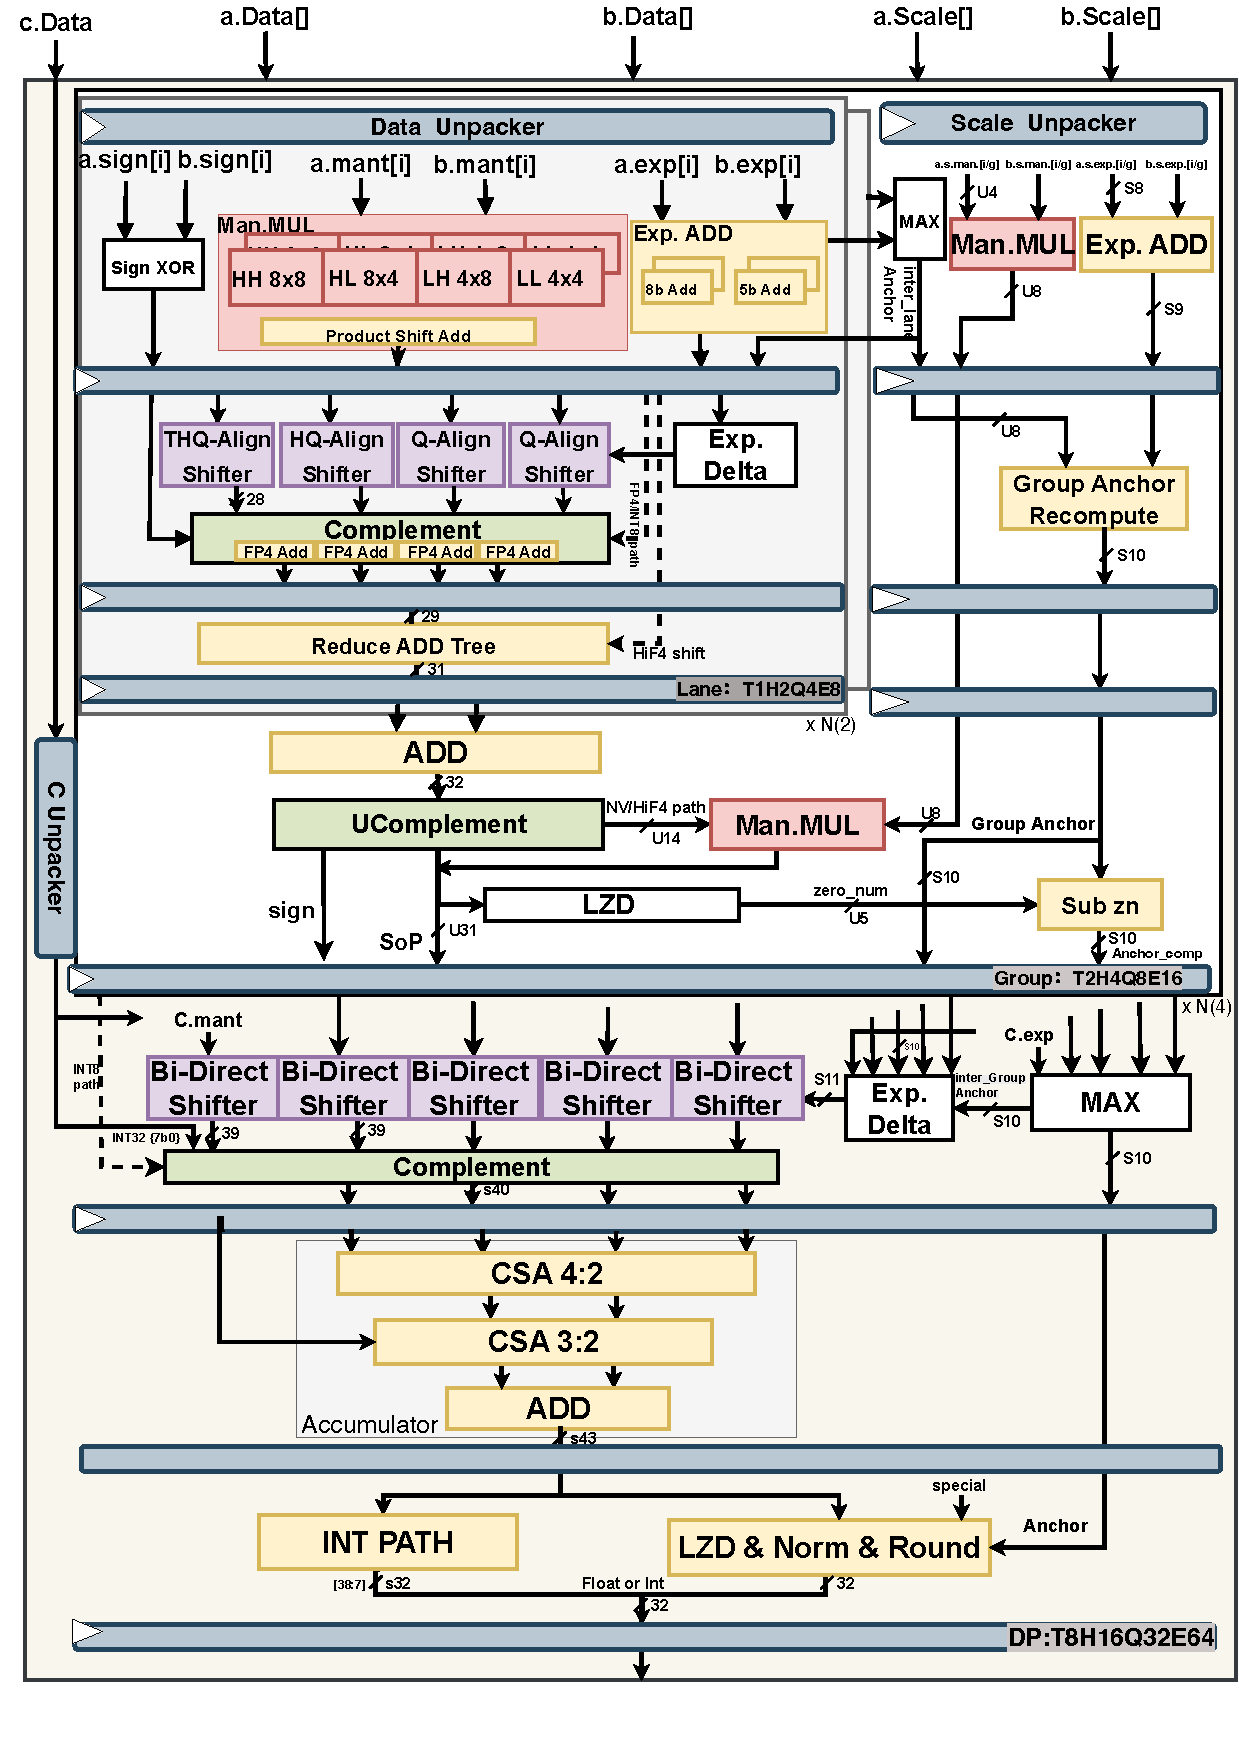
\includegraphics[width=\columnwidth]{baseline_arch.pdf}
\caption{Datapath of the $1:2:4$ baseline dot-product unit. Each Lane processes eight FP4 operand pairs per cycle because eight elements of each HiF4 input share a second-level micro-exponent. Two Lanes form a Group to match the 16-element block over which NVFP4 shares a scale factor.}
\label{fig:dp_architecture}
\end{figure}

The Lane decoder separates the sign from the unsigned multiplier input. For T, H, and Q, it extracts the exponent and restores the mantissa's implicit leading bit. The Q mantissa fits in four bits. For MXFP4 and NVFP4, folding the E2M1 exponent into the magnitude gives an exact four-bit fixed-point value with one fractional bit. For HiF4~\cite{hifloat4}, the first micro-exponent shifts the three-bit magnitude left to give a four-bit value with two fractional bits. The second micro-exponent scales the Lane sum. Q and E thus share unsigned $4\times4$ multiplication. INT8 uses the same unsigned datapath with a separate sign and an eight-bit magnitude.

Each Lane has two multiplier sets, each containing one $8\times8$, one $8\times4$, one $4\times8$, and one $4\times4$ multiplier. In TF32 and FP16 modes, shifting and adding the partial products within a set reconstructs the full mantissa product. In Q and E modes, the multipliers receive independent four-bit operands, producing four Q products or eight E products per Lane per cycle.

All modes share a four-input adder tree. T, H, and Q use one, two, and four shifters, respectively, to align products to the largest valid product exponent in the Group. Guided by the bit-width analysis in TensorGauge~\cite{tensorgauge} and reverse engineering of Blackwell FP8 arithmetic~\cite{xie2025mmasim}, we retain 26 fractional bits in the alignment window and truncate toward zero on right shifts. E and INT8 bypass the wide shifters. After sign restoration, the Lane reduces eight E products pairwise to four terms. The four INT8 products feed the tree directly.

Each Group combines its two Lane sums and applies block scaling. One Group covers a 16-element NVFP4 block, and multiple Groups share a scale for larger blocks. The power-of-two scales in MX formats adjust only the exponent. NVFP4 and HiF4 also require multiplication by the mantissas of both operand scales. Each Group outputs a sign, a 31-bit unsigned magnitude, and the exponent of its most significant physical bit. Leading-zero detection also gives the exponent of the highest nonzero bit for nonzero magnitudes. The DP uses the latter exponent to select a common alignment reference and the former to align each magnitude in one bidirectional shift. This interface accommodates format-specific binary-point positions while sharing the accumulation hardware.

\subsection{Low-Precision Group Specialization}
\label{sec:specialized_midgroups}

Each specialized Group retains the baseline decoding, alignment precision, and block-scaling rules for its supported formats. Each Lane in a Q8E16 Group uses eight $4\times4$ multipliers, activating four in Q mode and all eight in E mode, and the Group retains scale mantissa multiplication for NVFP4 and HiF4. Each Lane in a Q8 Group requires only four $4\times4$ multipliers and omits E decoding, micro-exponent handling, and scale mantissa multiplication.

E16 eliminates Group-wide element-exponent comparison and the wide alignment shifters in each Lane. A narrow adder tree reduces eight fixed-point products to a signed 14-bit Lane output, down from 31 bits in the baseline. After Group reduction and scaling, appending zeros at the least significant end maps the 22-bit magnitude to the 31-bit interface while preserving the bit weights of the baseline E path.

The stand-alone $0:2:4$ DP evaluated in Section~\ref{sec:evaluation} uses four Q8E16 Groups to process 32 Q pairs or 64 E pairs per cycle.

\subsection{Throughput-Ratio Composition and Fused Accumulation}
\label{sec:expansion}

Adding four E16 Groups to the baseline doubles E throughput alone ($1:2:8$). Adding four Q8E16 Groups doubles both Q and E throughput ($1:4:8$). Table~\ref{tab:ratio9_composition} lists the Group counts and resulting parallelism for all nine configurations.

% Group counts follow src/spec/dp/dptop/ mixed, Q-only, E192/E256,
% and QE192/QE256 expansion contracts. Ratios are normalized to H16.
% Single table source shared by the official and review manuscripts.
\begin{table}[t]
\centering
\caption{Group composition of the nine DP configurations}
\label{tab:ratio9_composition}
\begingroup
\footnotesize
\setlength{\tabcolsep}{2pt}
\begin{tabular*}{\columnwidth}{@{\extracolsep{\fill}}lrrrrl@{}}
\toprule
 H:Q:E & \shortstack{T2H4Q8E16\\Group} & \shortstack{Q8\\Group} & \shortstack{E16 \\ Group} & \shortstack{Q8E16\\Group} & \shortstack{Total DP\\parallelism} \\
\midrule
\tpratio{1}{2}{4}  & 4 & 0 & 0  & 0  & T8H16Q32E64   \\
\tpratio{1}{2}{6}  & 4 & 0 & 2  & 0  & T8H16Q32E96   \\
\tpratio{1}{2}{8}  & 4 & 0 & 4  & 0  & T8H16Q32E128  \\
\tpratio{1}{4}{4}  & 4 & 4 & 0  & 0  & T8H16Q64E64   \\
\tpratio{1}{4}{8}  & 4 & 0 & 0  & 4  & T8H16Q64E128  \\
\tpratio{1}{2}{12} & 4 & 0 & 8  & 0  & T8H16Q32E192  \\
\tpratio{1}{2}{16} & 4 & 0 & 12 & 0  & T8H16Q32E256  \\
\tpratio{1}{6}{12} & 4 & 0 & 0  & 8  & T8H16Q96E192  \\
\tpratio{1}{8}{16} & 4 & 0 & 0  & 12 & T8H16Q128E256 \\
\bottomrule
\end{tabular*}
\par\smallskip
\parbox{\columnwidth}{\raggedright
Group columns count instances; H:Q:E denotes the peak throughput ratio.
Total DP parallelism counts element pairs per cycle in mutually exclusive
T/H/Q/E modes.}
\endgroup
\end{table}


Each added Group has a bidirectional shifter. Active Groups participate in global exponent selection and apply scales at the original block boundaries. After alignment, a carry-save network reduces the added partial sums to two rows. A $4:2$ compressor merges these with the baseline rows, which already include the addend $C$. The accumulator width scales with the number of participating Groups. A precision-controlled multiplexer selects the baseline or merged sum and carry rows for a shared carry-propagate adder. Floating-point results are rounded to FP32 using round-to-nearest, ties-to-even. Inactive Groups are excluded from exponent selection and special-value reduction, preserving the baseline high-precision results. All configurations accept one independent request per cycle with an eight-cycle pipeline latency.
% END REVIEW PAIR: 03_architecture.tex

% BEGIN REVIEW PAIR: 04_evaluation.tex
\section{Evaluation}
\label{sec:evaluation}

% Generated by scripts/build_related_native.py; official manuscript.
\begin{table*}[!b]
\centering
\caption{Implementation conditions and efficiency at the reported process nodes}
\label{tab:related_dp}
\begingroup\footnotesize\setlength{\tabcolsep}{1.5pt}
\def\Eff#1{\begin{tabular}{@{}lr@{}}#1\end{tabular}}
\begin{tabular*}{\textwidth}{@{\extracolsep{\fill}}l*{7}{c}@{}}\toprule
Metric & Ten-Four~\cite{rout2026tenfourv3} & MPICC~\cite{huangMPICCMultiplePrecisionInterCombined2025} & MXDOTP~\cite{islamoglu2025mxdotp} & FPnew~\cite{mach2021fpnew} & MiniFloats~\cite{bertaccini2024minifloats} & \multicolumn{2}{c}{DP-Puzzle} \\
\cmidrule(lr){7-8}
 & & & & & &  \tpratio{1}{2}{4} & \tpratio{0}{2}{4} \\
\midrule
Structure & Fused DP & $n$-term MAC & MX DP & SIMD FMA & SIMD wDotp & MX DP & MX DP \\
Technology (nm) & 7 & 28 & 12 & 22 & 12 &  12 & 12 \\
Voltage (V) & 0.70 & 0.90 & 0.80 & 0.80 &  0.80 & 0.70 & 0.70 \\
Frequency (GHz) & 1.58 & 1.43 & 1.09 & 0.92 & 1.26 &  1.00 & 1.00 \\
Area ($\mu$m$^2$) & 2400 / 4650 & 2295 & 3150 & 49\,000 & 19\,000 & 16\,165.12 & 9\,762.99 \\
Accumulation & FP32/INT32 & FP12/INT8 & FP32 & Per format & FP16/FP32 &  FP32/INT32 & FP32 \\
\midrule
\shortstack[l]{Energy efficiency\\(TFLOP/s/W)} & --- & \Eff{FP8 & 1.95\\FP4 & 5.93} & \Eff{MXFP8 & 2.04} & \Eff{FP16 & 0.50\\BF16 & 0.58\\FP8 & 1.24} & \Eff{FP8 & 1.63\\FP16 & 0.82} & \Eff{BF16 & 2.09\\MXFP8 & 4.00\\MXFP4 & 11.43} & \Eff{MXFP8 & 5.23\\MXFP4 & 13.93} \\
\midrule
\shortstack[l]{Area efficiency\\(TFLOP/s/mm$^2$)} & \Eff{BF16 & 5.25 / 5.42\\MXFP8 & 10.50 / 10.84} & \Eff{FP8 & 1.25\\FP4 & 4.99} & \Eff{MXFP8 & 5.52} & \Eff{FP16 & 0.15\\BF16 & 0.15\\FP8 & 0.30} & \Eff{FP8 & 1.06\\FP16 & 0.53} & \Eff{BF16 & 1.98\\MXFP8 & 3.96\\MXFP4 & 7.92} & \Eff{MXFP8 & 6.56\\MXFP4 & 13.11} \\
\bottomrule\end{tabular*}
\par\smallskip
\endgroup
\end{table*}


\begin{figure*}[!t]
\centering
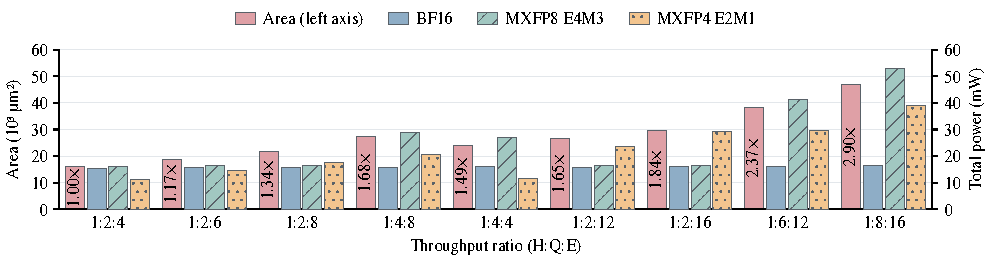
\includegraphics[width=\textwidth]{dp_ratio_area_power.pdf}
\caption{Synthesized area and total power across the evaluated throughput ratios. Area series use the left axis, with labels indicating ratios relative to $1:2:4$. The three power series share the right axis (mW). The labels are normalized to the outlined baseline MXFP8 bar.}
\label{fig:ratio4_costs}
\end{figure*}

\subsection{Experimental Setup and Verification}
\label{sec:eval_setup}
\label{sec:numerical_validation}

We implement the nine dot-product configurations in Verilog and verify their functionality using Verilator. All designs are synthesized and analyzed for timing using Synopsys Design Compiler in TSMC 12\,nm technology at the typical-typical (TT) corner (0.7\,V, 85$^\circ$C), targeting 1\,GHz with integrated clock gating enabled. The designs meet timing and electrical constraints. Area includes combinational logic, pipeline registers, and clock-gating cells. For power evaluation, we collect activations and weights from the first-layer multilayer perceptron (MLP) down-projection of Qwen3-8B running on WikiText-2~\cite{qwen3technicalreport,merity2016pointer}, and quantize them to BF16, MXFP8 E4M3, and MXFP4 E2M1. Power Compiler estimates total power using steady-state switching activity extracted from gate-level simulation at 1\,GHz. Area and power results correspond to synthesized dot-product units before clock-tree synthesis and place-and-route.

\subsection{Baseline Comparison with Prior Multi-Precision Units}
\label{sec:related_dp_evaluation}


Tables~\ref{tab:related_features} and~\ref{tab:related_dp} compare format coverage and implementation efficiency, respectively. Under the original published technology nodes and evaluation conditions, the DP-Puzzle $1:2:4$ baseline achieves $3.74\times$/$2.45\times$ the area/energy efficiency of MiniFloats at FP8. Separately, we use DeepScaleTool~\cite{sarangi2021deepscaletool} to scale Ten-Four from 7\,nm to 14\,nm as an approximate reference for our 12\,nm implementation. Under this estimate, our baseline achieves approximately $3\times$ the MXFP8 area efficiency of both full-format Ten-Four configurations.

Under the original-node comparison, the $0:2:4$ low-precision unit achieves $5.26\times$/$2.68\times$ the area/energy efficiency of MPICC at FP8 and $2.63\times$/$2.35\times$ at FP4. Compared with MXDOTP, also implemented at 12\,nm, it achieves $1.19\times$/$2.57\times$ the MXFP8 area/energy efficiency while additionally supporting MXFP4, NVFP4, and HiF4.

\subsection{Area and Power Across Throughput Ratios}
\label{sec:lowp_costs}

\textbf{Sharing low-precision hardware reduces the area cost of doubling both throughputs.} Relative to $1:2:4$, doubling MXFP8 alone ($1:4:4$) adds 48.56\% to DP area, and doubling MXFP4 alone ($1:2:8$) adds 33.60\% (Fig.~\ref{fig:ratio4_costs}). These increments sum to 82.16\% of baseline area. By reusing the same multipliers across modes in four added Q8E16 Groups, $1:4:8$ doubles both throughputs with 68.21\% more area, a 16.98\% saving on the combined incremental area.

\textbf{Maximum DP power grows modestly through $1:2:8$ and more sharply at $1:2:12$.} Relative to $1:2:4$, the maximum estimated DP power across the three modes rises by 9.95\% at $1:2:8$ and by 46.63\% at $1:2:12$. Doubling MXFP8 as well raises this maximum by 79.91\% at $1:4:8$, even though its MXFP4 throughput matches $1:2:8$. MXFP8 sets the maximum in the joint expansion, while MXFP4 sets it in both MXFP4-only expansions.

\textbf{Under joint MXFP8 and MXFP4 expansion, maximum mode power grows faster than DP area.} At $1:4:8$, $1:6:12$, and $1:8:16$, area reaches $1.68\times$, $2.37\times$, and $2.90\times$ the $1:2:4$ baseline, respectively, while maximum estimated power reaches $1.80\times$, $2.58\times$, and $3.30\times$ its baseline value. At $1:8:16$, each low-precision mode thus delivers 37.79\% more throughput per unit area. In MXFP8 mode, its estimated power per unit area is 13.78\% higher than that of the baseline.

% END REVIEW PAIR: 04_evaluation.tex

% BEGIN REVIEW PAIR: 05_dse.tex
\section{Case Study}
\label{sec:workload}

\begin{figure}[!t]
\centering
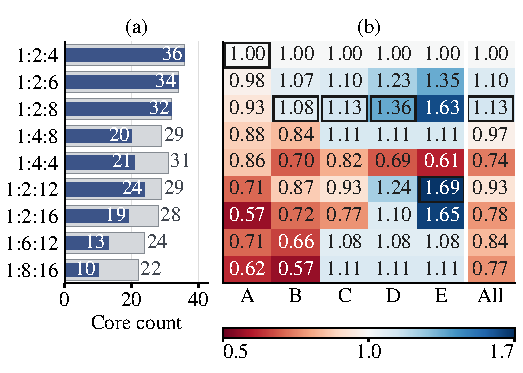
\includegraphics[width=\columnwidth]{v41_case_panels_overlay.pdf}
\caption{Fixed-budget comparison ($\alpha=0.327$, $\beta=1$). (a) Core counts under area-only (gray) and joint (blue) budgets. (b) Ideal GEMM compute speedups over $1:2:4$. A--E each aggregate 11 contexts. All aggregates 55 combinations with equal request weights. Outlines mark column maxima.}
\label{fig:fixed_budget_compact}
\end{figure}
We use DeepSeek-V4.1-Flash text prefill as a mixed-precision workload. Its released configuration defaults to FP8 for linear layers and uses FP4 weights for routed experts~\cite{deepseekv41source}. We examine how further precision changes in its GEMMs affect the preferred hardware throughput ratio under area and power limits.

\subsection{Deployment Scale Under Joint Budgets}
The $1:2:4$ baseline has $N_0=36$ cores, each with 256 DPs that accept one request per cycle at 1\,GHz. The parameter $\alpha$ is the DP-array fraction of baseline core area. Our reference $\alpha=0.327$ follows the reported Ascend Cube cluster area share~\cite{luo2024hifloat8area}. At each $\alpha$, the area budget is the area of $N_0$ baseline cores. We hold non-array area per core fixed across candidates. If candidate $j$ has $r_j$ times the synthesized DP area of the baseline, its core area is $1+\alpha(r_j-1)$ times the baseline core area.

We set the DP-array power cap to $\beta P_0$, where $P_0=N_0p_0$ is the baseline array power estimate. The per-core array power $p_j$ is 256 times the largest Power Compiler estimate for a single DP across BF16, MXFP8, and MXFP4. The feasible core count is
\begin{equation}
N_j(\alpha,\beta)=\min\!\left\{
\left\lfloor\frac{N_0}{1+\alpha(r_j-1)}\right\rfloor,
\left\lfloor\frac{\beta P_0}{p_j}\right\rfloor
\right\}.
\label{eq:joint_core_count}
\end{equation}

\subsection{GEMM Workload and Precision Migration}
% Workload evidence in ../paper/data/evidence/v41_five_stage_20261117/{manifest.json,operators.csv,cases.csv,gains.csv}.
We derive the GEMM counts from the model dimensions, expert assignments, and attention patterns. Each mixture-of-experts layer applies the gate, up, and down projections of six routed experts and one shared expert per token. The attention block adds the Q-up query projection and the grouped O-down and O-up output projections. Its $QK^{\mathsf{T}}$ and $PV$ products score keys and combine their values over the positions selected by sliding-window and compressed sparse attention. The three migration groups in Table~\ref{tab:five_stage_migrations} account for 68--94\% of the BF16, FP8, and FP4 GEMM work across the evaluated context lengths.

In reference scenario A, the routed experts use FP4 weights and FP8 activations (W4A8), so we model their work using FP8 throughput. The main attention products and grouped O-down use BF16. Scenarios B--E model progressively lower compute precisions at fixed operator shapes, motivated by routed-expert W4A4 quantization~\cite{nvidiav41routed2026} and low-precision attention~\cite{flashattention3,sageattention3}. The remaining GEMMs, including KV projections and the sparse indexer's FP4 score products, retain their reference precisions.
% Maps current A--E to previous A, B, D, E, F; no changes to operator shapes.
\begin{table}[t]
\centering
\caption{Five assumed precision-migration scenarios.}
\label{tab:five_stage_migrations}
\begingroup\footnotesize\setlength{\tabcolsep}{4pt}
\begin{tabular}{@{}cccc@{}}\toprule
Case & \shortstack{Routed\\experts} & \shortstack{Shared experts\\+ Q-up/O-up} & \shortstack{Main QK/PV\\+ Grouped O-down} \\\midrule
A & FP8 & FP8 & BF16 \\
B & FP4 & FP8 & BF16 \\
C & FP4 & FP8 & FP8 \\
D & FP4 & FP4 & FP8 \\
E & FP4 & FP4 & FP4 \\\bottomrule
\end{tabular}
\par\vspace{2pt}\begin{minipage}{0.98\columnwidth}\footnotesize
Experts include gate/up/down; Main QK/PV includes SWA/CSA.
Each stage retains earlier migrations; other operators keep their original precision.
\end{minipage}
\endgroup
\end{table}


We evaluate batch-one cold prefill at 11 doubling context lengths from 1K to 1M tokens. With full array utilization and sufficient data supply, we estimate GEMM compute time for request $k$ as $\sum_p F_{k,p}/(N_jR_{j,p})$. We map the BF16, FP8, and FP4 operation counts $F_{k,p}$ to the per-core peak rates $R_{j,p}$ of the BF16, MXFP8, and MXFP4 modes, respectively, and track FP32 work separately. Speedup is the $1{:}2{:}4$ baseline's mean time divided by the candidate's mean under the same budgets, with equal weight for all 55 scenario--context combinations.

At $(\alpha,\beta)=(0.327,1)$, $1{:}2{:}8$ fits 32 cores, and the power cap reduces $1{:}8{:}16$ from 22 area-limited cores to 10 (Fig.~\ref{fig:fixed_budget_compact}(a)). The best ratio shifts from $1{:}2{:}4$ in A to $1{:}2{:}8$ in B--D and $1{:}2{:}12$ in E. Across all five scenarios, $1{:}2{:}8$ gives the highest aggregate GEMM compute speedup of $1.13\times$ (Fig.~\ref{fig:fixed_budget_compact}(b)).

% Scan evidence: build/v41_joint_budget_dse_extended/{scan.py,manifest.json,summary.json}.
\begin{figure}[!t]
\centering
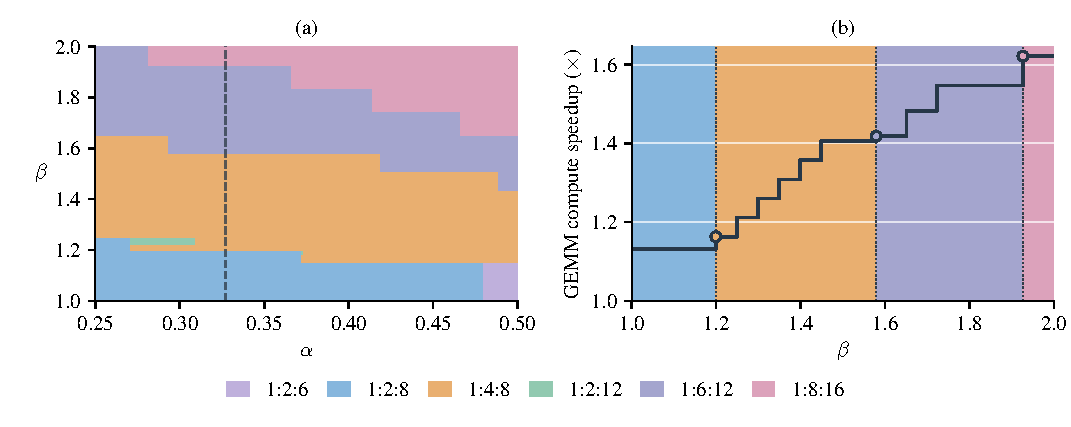
\includegraphics[width=\columnwidth]{joint_budget_dse_extended.pdf}
\caption{Joint-budget sweep for five migration scenarios and 11 contexts. (a) Throughput ratio minimizing mean modeled GEMM compute time at each $(\alpha,\beta)$. (b) GEMM compute speedup over the same-budget $1:2:4$ baseline along the dashed $\alpha=0.327$ slice. Colors identify selected ratios. Markers denote switches at $\beta\approx1.1994$, $1.5792$, and $1.9267$.}
\label{fig:budget_dse_extended}
\end{figure}

\subsection{Throughput-Ratio Boundaries Under Joint Budgets}
Fig.~\ref{fig:budget_dse_extended}(a) shows which ratio minimizes mean GEMM compute time over $\alpha\in[0.25,0.50]$ and $\beta\in[1,2]$, with integer core counts given by~\eqref{eq:joint_core_count}.

\textbf{Tight power budgets favor moderate MXFP4 expansion.} At $\beta=1$, $1{:}2{:}8$ leads across most of the area sweep, up to $\alpha\approx0.48$. Its added MXFP4 throughput is paired with enough deployed cores to serve the remaining mixed-precision work. Larger expansions become competitive as the power cap admits more cores. At $\alpha=0.50$, the best speedup levels off after the winning design reaches its area-limited core count.

\textbf{A ratio switch sets a power target for further expansion.} At the reference area, the first switch needs about 20\% more array-power budget to admit the 24th $1{:}4{:}8$ core (Fig.~\ref{fig:budget_dse_extended}(b)). At fixed area and peak rates, fitting those 24 cores at $\beta=1$ would require about 16.6\% lower maximum-mode array power per core. This threshold gives a concrete power target for adding MXFP8 and MXFP4 throughput under a fixed budget.
% END REVIEW PAIR: 05_dse.tex

% BEGIN REVIEW PAIR: 06_conclusion.tex
\section{Conclusion}
\label{sec:conclusion}
DP-Puzzle combines shared multi-precision dot-product datapaths with precision-specific Groups to construct nine throughput ratios. Synthesis and activity-driven power evaluation quantify their implementation costs and efficiency, supporting chip-level throughput modeling under common area and power budgets. Under the budgets and precision-migration assumptions of our case study, moderate low-precision expansion balances deployment density and mixed-precision demand, providing guidance for throughput-ratio selection as workloads evolve.
% END REVIEW PAIR: 06_conclusion.tex


\section*{Content Generated by AI}
OpenAI Codex assisted with RTL testing, debugging, performance optimization, and EDA scripting. It also assisted with modeling, data analysis, and plotting for Sections~\ref{sec:evaluation} and~\ref{sec:workload}, and with manuscript drafting, translation, and editing. The authors take full responsibility for the paper and its results.

\clearpage
\setcounter{DACreferencepage}{\value{page}}
\ifnum\value{DACreferencepage}>7\relax
  \PackageWarningNoLine{DAC2027}{Main text exceeds six pages}%
\fi
\typeout{DAC2027: References start on page \thepage}
\bibliographystyle{IEEEtran}
\bibliography{references/references}
\end{document}
